\chapter{Unidade de Processamento Gráfico}\index{GPU}\label{GPU}

    A GPU nasceu da necessidade de renderizar cenas complexas, mantendo uma taxa de quadros por segundos
aceitável para o usuário, em tempo real. Ela foi projetada para executar uma sequência fixa de passos que transformam
os dados da cena em objetos virtuais na tela. A sequência de passos se assemelha a uma linha de montagem de fabricas,
onde objetos são montados parte por parte de forma sequencial. Chamamos essa sequência de \textit{Pipeline} gráfico
(ver figura \ref{fig:pipeline}), e a GPU é construída para que cada passo dele seja mapeado para uma ou mais partes do
seu hardware.

    É comum cenas conterem objetos complexos, compostos de milhões de triângulos, que passarão, um por um, pelo
\textit{Pipeline} gráfico. Para acelerar o processo de renderização, as GPUs seguem a arquitetura de Instrução Única,
Múltiplos Dados (\textit{Single Instruction, Multiple Data} - SIMD). Como o nome já diz, essa arquitetura permite que
a mesma instrução seja executada várias vezes em paralelo utilizando instâncias de dados diferentes. A figura
\ref{fig:simd} mostra a implementação do \textit{Pipeline} utilizando a arquitetura SIMD no hardware da GPU.

  Para atingir um desempenho satisfatório utilizando o paradigma SIMD, o hardware
da GPU é especialmente construido para facilitar o abundante paralelismo. Os
processadores são agrupados em blocos fisicos chamados de \textit{Streaming Multiprocessors} (SM),
compostos de, além dos processadores, um bloco pequeno de memória compartilhada,
um conjunto de registradores e unidades de processamento gráficos, cada uma criada
com a finalidade de agilizar o processamento de funções usadas comumente no pipeline
gráfico. A GPU conta, ainda, com uma unidade de escalonamento, que é responsável
por distriur as \textit{threads} entre todos os SMs disponiveis.

    O código que será executado em cada processador é chamado de \textbf{kernel}. Ao executar um \textbf{kernel} na GPU, o
hardware criará \textit{threads}, cada uma delas executando o mesmo código, mas com dados diferentes. Nas placas NVIDIA as \textit{threads}
são agrupadas em blocos, e esses blocos são escalonados para cada SM. Depois, todas as \textit{threads} dentro de um bloco são
divididas em pequenos grupos chamados de \textbf{warp}, e cada warp é executado paralelamente dentro do
mesmo SM para qual o bloco foi escalonado, onde cada \textit{thread} dentro de um \textit{warp} executa a mesma linha de código ao mesmo tempo.
Existe um limite para a quantidade de \textit{threads} escalonadas para execução
dentro de um SM, que é definida pelos recursos que cada \textit{thread} consome. Por exemplo, não há como executar 10 \textit{threads}
que consomem 10 registradores cada em um SM com 90 registradores.

    A memória da GPU é limitada em relação à da CPU. O acesso a um mesmo bloco de memória é concorrente, mas ao utilizar caches e leitura
ou escritas em conjunto podemos minimizar a taxa com que leituras ou escritas conflitantes são feitas. Mas ainda sim é
necessário atenção ao construir um kernel. Dada a estrutura do hardware da GPU, é melhor deixar \textit{threads} que façam
operações sobre posições de memória próximas no mesmo SM, dado que cada requisição
a uma posição da memória principal retorna um bloco, e não uma posição especifica.

    Outro fator limitante é a transferência de dados da memória principal do computador para a memória
principal da GPU. A transmissão é feita por um barramento PCI Express, com velocidades de até 16GB/s.
Dada a presença dessa lentidão, é aconselhável manter pelo maior tempo possivel
os dados na GPU, mesmo que isso implique na execução de trechos de código que não
sejam altamente paralelizáveis.

\begin{figure}[H]
    \centering
    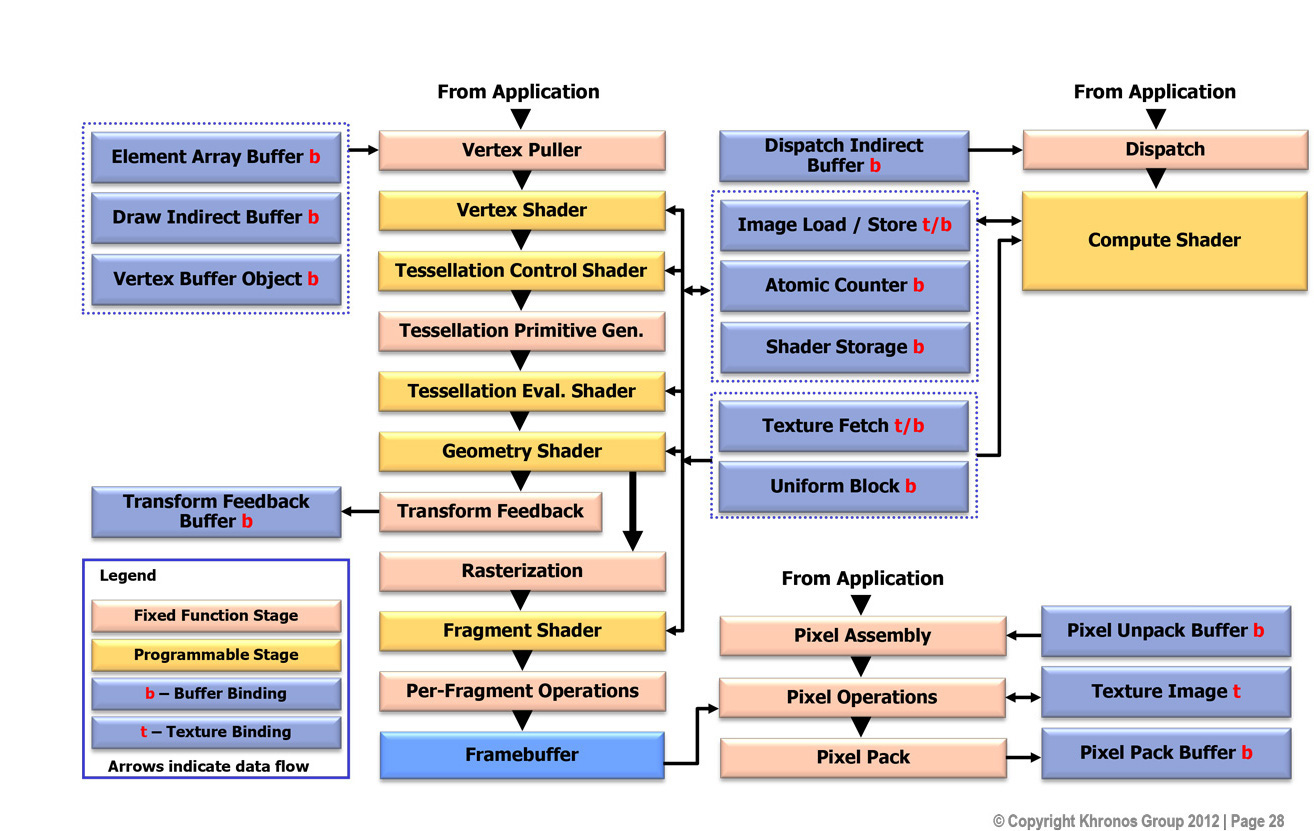
\includegraphics[width=1\textwidth]{figuras/pipeline.jpg}
    \caption{\textit{Pipeline} do OpenGL 4.x, por \citep{pipeline}. Todos os passos marcados pela cor amarela podem
    ser reprogramados para serem utilziados por aplicações GPGPU. (Modificada)}
    \label{fig:pipeline}
\end{figure}

\begin{figure}[H]
    \centering
    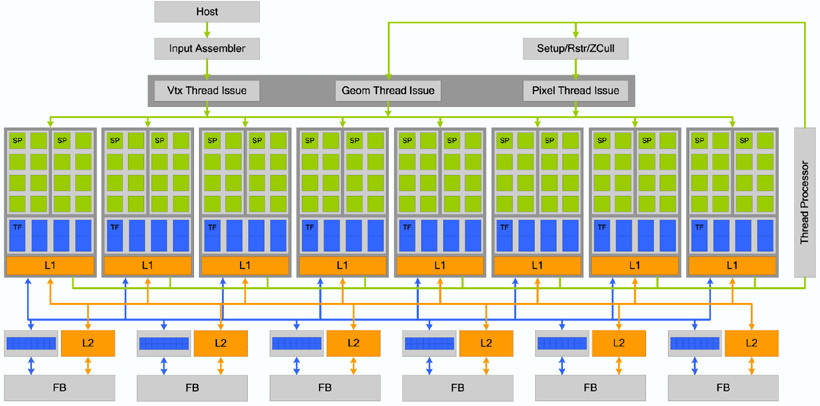
\includegraphics[width=1\textwidth]{figuras/simd.jpg}
    \caption{Arquitetura da GPU SIMD, por \citep{blythe2008rise}.}
    \label{fig:simd}
\end{figure}

\section{CUDA}\index{CUDA}
\textit{Compute Unified Device Architecture}, definida pela (CUDA) é uma arquitetura de programação para GPUs criada
pela ~\cite{nvidia2007compute}.
Ele adiciona diretrizes para as linguagens C, C++, FORTRAN e Java, permitindo que elas usem a GPU.
A versão 1.0 do CUDA foi disponibilizada no inicio de 2007. Atualmente só existe um compilador para CUDA, o nvcc,
e ele só da suporte para GPUs NVIDIA. Existe uma separação clara entre os dois
ambientes de execução do código. Chamamos de \textit{Host} a CPU, e de \textit{Device}
a GPU. Um \textit{kernel} só é executado atrávez de uma chamada originada do \textit{Host}.

O CUDA implementa um conjunto virtual de instruções e memória, tornando os programas retroativos. O compilador
primeiro compila o código em C para um intermediário, chamado de PTX, que depois será convertido em linguagem
de máquina. Na conversão do PTX para linguagem de máquina o compilador verifica quais instruções o \textit{device}
suporta e converte o código para usar as instruções corretas.
Para obter o maior desempenho possível, é importante saber para qual versão o código final será compilado,
pois na passagem do código de uma versão maior para uma menor não existe a garantia que o algoritmo seguira as mesmas instruções,
o compilador pode mudar um conjunto de instruções para outro menos eficiente, ou em alguns casos, algumas instruções não existem em
versões mais antigas do hardware.

\subsection{Modelo de Plataforma}
A inicialização dos recursos que o CUDA necessita para a comunicação com a GPU é feita no background da
aplicação no momento da primeira chamada de alguma das diretivas do CUDA. Essa primeira diretiva terá um
tempo maior de execução que chamadas subsequentes a mesma diretiva. Na inicialização o CUDA identifica
os \textit{devices} existentes e escolhe um deles para ser o responsável pelas execuções posteriores.

O próximo passo é a alocação de memória no \textit{device}. As operações de leitura de memória de um kernel são feitas somente
na memória de um \textit{device}. A alocação dessa memória é feita pelo \textit{host}, usando \codepagode{codaMalloc()}.
Para copiar a memória do \textit{host} para o \textit{device} ou vice-versa,
\codepagode{cudaMemcpy()} é usada. Para liberar o espaço alocado após a execução basta usar o \codepagode{cudaFree()}.
Todas essas diretivas recebem um ponteiro do \textit{host}, usado para o controle sobre qual posição da memória está sendo
operado em cada operação.

O CUDA dá suporte a alocação de vetores em duas ou três dimensões através de: \codepagode{cudaMallocPitch()} e
\codepagode{cudaMalloc3D()}, respectivamente. É necessário usar as modificações dos comandos \codepagode{Memcpy} para
duas ou três dimensões também, que são: \codepagode{cudaMemcpy2D()}, \codepagode{cudaMemcpy3D()}.

\subsection{Modelo de Programação}
Um kernel no CUDA é uma função C que será executada paralelamente $n$ vezes em $n$ \textit{threads} diferentes na GPU. Um kernel pode ser
definido em qualquer lugar do seu código, usando a declaração \codepagode{\_\_global\_\_} do lado esquerdo do tipo de retorno do kernel.
Para invocar um kernel, o \textit{host} faz a chamada de uma função com a sintaxe parecida com o C, mas usa uma configuração de
execução definida pelo CUDA, que usa a sintaxe \verb#<<<...>>># junto da chamada da função. Os parâmetros da configuração são
o número de blocos de \textit{threads} e o número de \textit{threads} por blocos. Para somar dois vetores de tamanho M e guardar o resultado num
outro vetor, o código é o seguinte:

\begin{lstlisting}
  __global__ void MatrixMulti ( float* a, float* b, float* c) {
    int i = threadIdx.x;
    a[i] = b[i] + c[i];
  }

  int main () {
    ...
    VecAdd<<<1,M>>>(a, b, c)
    ...
  }
\end{lstlisting}

No kernel acima, a linha \codepagode{int i = threadIdx.x} atribui a variável i o valor do índice da \textit{thread} em execução.
A estrutura \codepagode{threadIdx} é um vetor de 3 dimensões, logo as \textit{threads} podem ser organizadas em 1, 2 ou 3 dimensões dentro de um
\textit{device}. As \textit{threads} são organizadas por blocos. Cada bloco tem dimensões maleáveis. Blocos são organizados em
grids, que tem seu tamanho configurado na chamada o kernel, bem como o tamanho de cada bloco. No nosso exemplo acima, na linha
\verb#VecAdd<<<1,M>>>(a,b,c)#, o 1 determina o número de blocos e o M o número de \textit{threads} por bloco.
O CUDA supõem que todos os blocos podem ser executados de maneira independente,
ou seja, nem sempre os blocos são executados seguindo seus índices.

O CUDA utiliza o Compute Capability (Capacidade Computacional) do \textit{device} no qual ele irá executar o \textit{kernel}
para identificar quais instruções ele pode utilizar. A Compute Capability de um \textit{device}
representa a arquitetura do \textit{device}, e outro que representa melhorias numa arquitetura.
A arquitetura \textit{Tesla}, a primeira da NVIDIA a dar suporte a GPGPU, tem Compute Capability 1.x, a seguinte, a \textit{Tesla},
tem 2.x e a atual, a \textit{Kepler}, tem 3.x. Dentro de cada arquitetura, podem existir melhorias nas instruções, que são
refletidas no número após o ponto, ou seja, uma placa com Compute Capability 2.1 tem instruções que uma 2.0 não tem.

\subsection{Hierarquia de Memória}
No CUDA, a memoria é separada em 3 locais:

\begin{itemize}
  \item Registradores - Todas as variáveis de uma \textit{thread} fica em registradores.
  \item Memória Compartilhada - Cada bloco de \textit{threads} tem uma memória compartilhada. A memória compartilhada é separada em
          pequenos blocos independentes. A memória compartilhada fica em chips dentro dos SMs, logo seu acesso é mais rápido do que o acesso a
          memória global.
  \item Memória Global - A memória global é acessível por qualquer bloco em execução em um \textit{device}.
        Leituras feitas na memória global apresentam a maior latência quando comparadas às anteriores.
        Toda transação feita na memória global é alinhada via 32, 64 ou 128 bytes.

\end{itemize}

Por padrão, o compilador do CUDA cuida do gerenciamento da memória, ou seja, ele é o responsável por distribuir os dados
entre os locais diferentes de memória. O programador pode dar dicas para o compilador usando qualificadores indicando o local
que ele quer que aquele elemento fique na memória. Os possíveis qualificadores são:
\begin{itemize}
  \item \codepagode{\_\_device\_\_} Fica na memória global.
  \item \codepagode{\_\_constant\_\_} Fica na area constante da memória global.
  \item \codepagode{\_\_shared\_\_} Fica na memória compartilhada das \textit{threads}.
  \item \codepagode{\_\_restrict\_\_} Indica para o compilador que todos os ponteiros com esse qualificador apontam para locais diferentes
                            da memória. Isso é importante pois o compilador pode fazer otimizações com o código sabendo dessa informação.
\end{itemize}

GPUs com Compute Cabapility maior ou igual a 2.0 podem alocar memória dentro do \textit{device} em tempo de execução.
